\documentclass[aps,pra,reprint,superscriptaddress,nofootinbib,floatfix]{revtex4-2}
\usepackage{amsmath,amssymb,bm,graphicx}
\usepackage[colorlinks=true,linkcolor=blue,citecolor=blue,urlcolor=blue]{hyperref}
\newcommand{\spec}{\operatorname{spec}}
\newcommand{\Tr}{\operatorname{Tr}}
\newcommand{\ii}{\mathrm{i}}
\renewcommand{\theequation}{S\arabic{equation}}
\renewcommand{\thefigure}{S\arabic{figure}}
\begin{document}
\title{Supplemental Material: Observable-dependent relaxation near a fermionic Liouvillian exceptional point}
\hypersetup{pdftitle={Supplemental Material: Observable-dependent relaxation near a fermionic Liouvillian exceptional point}}
\maketitle

\section{Exact observable projections}
The diagonal operator space can be identified with $n$ Boolean spins, one for the occupation of each energy eigenmode. In this space, the recycling generator is $G_{n,d}=J_-+zJ_+^d/d!$. In the basis of unnormalized particle-number projectors $P_k$, its maximal-spin matrix $N_{n,d}(z)$ has entries
\begin{equation}
N_{k-1,k}=n-k+1,\qquad N_{k+d,k}=z\binom{k+d}{d}.
\label{eq:N}
\end{equation}
These are coefficients per configuration. The aggregate-population matrix in the main text is
\begin{equation}
B_{n,d}=W_nN_{n,d}W_n^{-1},\qquad
(W_n)_{kk}=\binom nk.
\label{eq:weight}
\end{equation}
The binomial factors are essential when calculating probabilities or expectation values.

For $D=n_1-n_2$, let $m=n-2$ and $Q_k=DP_{k+1}$. The two marked Boolean spins form the singlet $|10\rangle_B-|01\rangle_B$, while the other $m$ spins are symmetric. Thus $Q_k=J_+^kQ_0/k!$ and
\begin{align}
J_-Q_k&=(m-k+1)Q_{k-1},& J_+Q_k&=(k+1)Q_{k+1},\nonumber\\
\Tr Q_k&=\Tr(\hat NQ_k)=0,& \Tr(DQ_k)&=2\binom mk.
\label{eq:identities}
\end{align}
The span of the $Q_k$ is one spin-$m/2$ copy. Since it is invariant under both $J_+$ and its transpose $J_-$, its orthogonal complement in the Boolean space is also invariant. As $D=\sum_kQ_k$, other spin copies do not contribute to this observable.

For an arbitrary initial density matrix define the aggregate projections
\begin{equation}
u_k=\Tr(P_k\rho_0),\qquad v_k=\Tr(DP_{k+1}\rho_0).
\end{equation}
Writing $E_M(t)=e^{\gamma t B_{M,d}(z)}$, the exact signals are
\begin{align}
\langle\hat N\rangle_t&=\frac{\bm k^TE_n(t)u}{\bm1^TE_n(t)u},\nonumber\\
\langle D\rangle_t&=\frac{\bm1^TE_m(t)v}{\bm1^TE_n(t)u},\qquad
P_{\rm surv}=e^{-n\gamma t}\bm1^TE_n(t)u,
\label{eq:general}
\end{align}
where $\bm k=(0,1,\ldots,n)^T$. Off-diagonal energy-basis operators remain in complementary invariant blocks and have zero trace against these diagonal observables.

For $\rho_0=\rho_p(1+\epsilon D)$, the two projections become
\begin{align}
u_k&=\binom nk p^k(1-p)^{n-k},\nonumber\\
v_k&=2\epsilon\binom mk p^{k+1}(1-p)^{n-k-1}.
\end{align}
This proves the two formulas in the main text. The positivity of $u$, and positivity of $\operatorname{sgn}(\epsilon)v$, guarantee their Perron overlaps when the corresponding matrices are irreducible. At $p=0.75$, $\epsilon=0.6$, $\langle D\rangle_0=0.225$ and $\langle\hat N\rangle_0=0.75n$.

To specify the particle-number rate without a generic-overlap shortcut, let $r_j,l_j$ be right and left eigenvectors of $B_{n,d}(z)$ at a simple root $\mu_j$, with $l_j^\dagger r_j=1$. Set $\mu_*=q\kappa_{n,d}$ and $\nu_*=(\bm k/n)^Tr_*/(\bm1^Tr_*)$. Then
\begin{equation}
C_j=(\bm k/n-\nu_*\bm1)^Tr_j\,l_j^\dagger u.
\end{equation}
The conditional rate uses the largest $\Re\mu_j$ for which $C_j\ne0$, with $j\ne *$. The denominator's leading amplitude $(\bm1^Tr_*)(l_*^\dagger u)$ is strictly positive for any physical nonzero $u\ge0$. A nonzero numerator is a separate requirement. For real simple first and second roots,
\begin{equation}
A_N=\frac{C_1}{(\bm1^Tr_*)(l_*^\dagger u)},\qquad
A_D=\frac{(\bm1^Tr_{m,*})(l_{m,*}^\dagger v)}{(\bm1^Tr_*)(l_*^\dagger u)}.
\end{equation}
The reported theoretical curves use these projections, not fitted amplitudes. Only the relevant simple roots are projected: inverting a complete eigenvector matrix would be invalid in the presence of a residual zero Jordan block.

If $m<d$, the imbalance block contains only lowering transitions. The positive initial state has a nonzero highest-weight component, so its numerator has degree $m$ in time. Its long-time form is $A_Dt^me^{-\gamma q\kappa_{n,d}t}$, not a pure exponential. Complex visible roots likewise require oscillatory factors. These cases do not invalidate the exact expressions~\eqref{eq:general}.

Observable-sector selection is a pre-existing mechanism~\cite{vanCaspel}. The present specialization provides exact fermionic channels and their conditional normalization. Fermion-parity evenness means $\Pi\rho\Pi=\rho$, not exclusive support on even particle numbers. One-time even-state/even-observable signals have no odd component. A two-time fermionic correlator can have an odd intermediate insertion, and is outside that exclusion.

\section{Complete fermionic blocks and gaps}
Diagonalize the number-conserving quadratic Hamiltonian. Both the uniform loss channels and all uniform $d$-creation channels are invariant under this rotation; the latter statement uses unitarity of the exterior-power representation. Let $A,B$ be disjoint ket-only and bra-only occupied sets and $C$ a common occupied subset of the remaining $m=n-|A|-|B|$ modes. The operators $|A\cup C\rangle\langle B\cup C|$ have Hamiltonian shift $-\ii(E_A-E_B)$. Multiplication by
\begin{equation}
g_{A,B}(C)=(-1)^{\sum_{c\in C}|\{f\in A\cup B:f<c\}|}
\end{equation}
removes the fermionic signs from every recycling edge. The block is
\begin{equation}
[-n\gamma-\ii(E_A-E_B)]\mathbb1+\gamma G_{m,d}.
\end{equation}
The spin-$s=(m-2j)/2$ component of $G_{m,d}$ is similar to $N_{m-2j,d}$ and hence to $B_{m-2j,d}$. Its multiplicity is $\eta_{m,j}=\binom mj-\binom m{j-1}$. The full multiset spectrum is
\begin{equation}
\biguplus_{\substack{A\cap B=\varnothing\\0\le j\le\lfloor m/2\rfloor}}
\left[-n\gamma-\ii(E_A-E_B)+\gamma\spec B_{m-2j,d}(z)\right]^{\eta_{m,j}}.
\label{eq:full}
\end{equation}
The Hamiltonian shifts do not affect real-part gaps. Quadratic-fermion Jordan theory~\cite{Prosen} does not directly diagonalize the $d>1$ recycling term; the uniform-channel representation is used here.

For $m\ge d$, the directed Boolean graph of $G_{m,d}$ is irreducible. Any set can lose all its particles; from the empty set one can construct any set by additions of $d$ particles and removals of the surplus. Its Perron vector is unique and permutation invariant, hence belongs to maximal spin. The subspace of subsets not containing an added mode gives $G_{m,d}$ as a principal submatrix of $G_{m+1,d}$. Perron monotonicity then orders the block edges. Parity-even operators require $|A|+|B|$ even, and the largest competing edge has effective size $n-2$ rather than $n-1$. Competition with the maximal block's own subleading roots yields the two exact minimum formulas in the main text.

For $n=d=4$, $N_{4,4}(1)^5=24\mathbb1$. Its subleading fifth roots have real part $24^{1/5}\cos(2\pi/5)>0$, whereas $\kappa_{3,4}=\kappa_{2,4}=0$. Thus the internal complex roots control both gaps, and the $D$ numerator has a quadratic time prefactor. This physical counterexample ($z=1\le4$) rules out a universal identification of $\Gamma_D$ with $\Delta_{\rm even}$.

\section{Polynomial truncation and established spectral structure}
The main text uses exact finite matrices throughout. For completeness we retain the characteristic-polynomial clarification that motivated the earlier spectral analysis of the model~\cite{XuYi}. Define $p_\ell(\mu,z)$ as the determinant of the first $\ell$ rows and columns of $\mu\mathbb1-N_{n,d}(z)$, with the full $n$ fixed. Then $p_0=1$, $p_\ell=\mu^\ell$ for $1\le\ell\le d$, and
\begin{align}
p_\ell&=\mu p_{\ell-1}-z w_{\ell-d-1}p_{\ell-d-1},\nonumber\\
w_i&=\binom{i+d}{d}\frac{(n-i)!}{(n-i-d)!}.
\end{align}
A nontrivial cycle in a determinant permutation occupies a consecutive interval of length $d+1$. The disjoint-interval expansion gives
\begin{equation}
p_{n+1}=\sum_{j=0}^{\lfloor(n+1)/(d+1)\rfloor}(-z)^jW_j\mu^{n+1-(d+1)j},\qquad W_j>0,
\label{eq:poly}
\end{equation}
where $W_0=1$. Coefficients of this type and all-orders leading splitting polynomials are established in structured-Jordan perturbation theory~\cite{MaEdelman}; higher-spin perturbations and eigenvalue rings also have direct precedents~\cite{Graefe}.

With $q=z^{1/(d+1)}$, the diagonal similarity $\mathsf D_{kk}=q^k$ gives $\mathsf D^{-1}N(z)\mathsf D=qN(1)$. Thus every nonzero eigenvalue has exact fractional scaling. McMillen's theorem~\cite{McMillen} gives distinct positive radii $\rho_a$ and simple nonzero roots $\rho_a e^{2\pi\ii j/(d+1)}$. The zero algebraic multiplicity is $r=(n+1)\bmod(d+1)$. The matrix is cyclic, since its transpose is unreduced upper Hessenberg; for $r>0$, the residual zero generalized eigenspace is one size-$r$ Jordan block.

For $n=7,d=2$, one obtains
\begin{equation}
p_8=\mu^8-504z\mu^5+27504z^2\mu^2.
\end{equation}
There are two cubic triplets and one size-two zero Jordan block (Fig.~\ref{fig:splitting}). The linear truncation gives one triplet and five zero roots. At fixed nonzero $\mu$, the discarded term is $O(z^2)$; at $\mu=qx$, every term in Eq.~\eqref{eq:poly} is proportional to $q^{n+1}$. The truncation is nonuniform on the splitting scale. Higher powers first occur at $n+1\ge2(d+1)$.

Eq.~(54) of Xu and Yi~\cite{XuYi} uses an approximate-equality sign (arXiv v2 numbering; Eq.~(49) in v1). This observation limits extraction of the full root pattern from that truncation; it does not overturn their exponent. Their Fig.~2 uses $n=4$, where the truncation is complete for $d=2,3,4$, while Appendix C separately solves $d=1$. Those tests are not contradicted. Publication metadata were verified; the equation-by-equation check uses arXiv v2 because the publisher PDF was not accessible.

\begin{figure}[!htb]
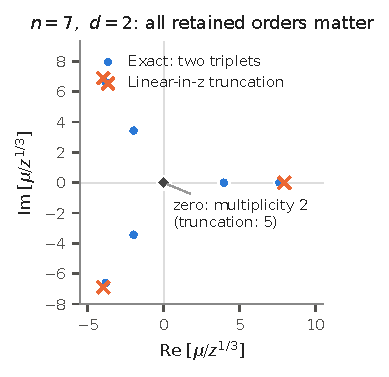
\includegraphics[width=.88\columnwidth]{../figs/splitting.pdf}
\caption{Exact scaled roots for $n=7,d=2$ and the linear-in-$z$ truncation. The discrepancy is independent of $z>0$ after dividing out $z^{1/3}$. The exact residual zero multiplicity is two.}
\label{fig:splitting}
\end{figure}

\section{Semiclassical expansion and its limits}
Let $s=n/2$ and use the orthonormal spin representation $\mathsf N_s=J_-+zJ_+^d/d!$. With $S=e^{\eta J_z}$ and $e^{(d+1)\eta}=zs^{d-1}/(d-1)!$,
\begin{equation}
S^{-1}\mathsf N_s S=e^\eta T_s,\qquad
T_s=J_-+\frac{J_+^d}{d s^{d-1}}.
\end{equation}
Around the $+x$ direction, set $J_x=s-Q$, $Q=b^\dagger b=(X^2+P^2-1)/2$, $[X,P]=\ii$, and $J_y=\sqrt{s}X+O(s^{-1/2})$. Keeping noncommutative operator ordering gives
\begin{align}
T_s&=s(1+1/d)+H_0+s^{-1/2}V_3+O(s^{-1}),\nonumber\\
H_0&=1-P^2-\frac{d+1}{2}X^2,\nonumber\\
V_3&=-\ii(d-1)\left[\frac{\{X,Q\}}2+\frac{d-2}{6}X^3\right].
\end{align}
The constant $+1$ comes from $-2Q=1-X^2-P^2$. The leading odd operator $V_3$ has zero diagonal expectation in oscillator eigenstates. Its second-order correction enters at $O(s^{-1})$, together with the next even operator. Since $e^\eta=q a_dn^{\beta_d}$, the oscillator levels $1-(2\ell+1)\Omega_d$ give the edge expansion in the main text.

Independently, the discrete ansatz $v_k\sim e^{nS(k/n)}$ at $z=\zeta n^{1-d}$ gives
\begin{equation}
\frac{\mu}{n}=(1-x)e^p+\frac{\zeta x^d}{d!}e^{-dp},\qquad p=S'(x).
\end{equation}
Minimizing over real $p$ and maximizing the envelope over $x$ yields $x_*=1/2$ and $\mu/n\sim C_d\zeta^{1/(d+1)}$, where
\begin{equation}
C_d=(d+1)d^{-d/(d+1)}(d!)^{-1/(d+1)}4^{-d/(d+1)}.
\end{equation}
The saddle location is not an assertion that the conditional particle filling is one half: the coefficient vector and population vector differ by Eq.~\eqref{eq:weight}.

These are formal fixed-$d$, fixed-low-excitation asymptotics. The expansion is not a global operator-norm estimate. McMillen's exact rays exclude off-axis edge competitors, whose real-part separation is of order $n^{\alpha_d}$ rather than $n^{\beta_d}$. They do not prove that the first two positive radial roots coincide with the local oscillator levels, or a uniform remainder bound. The latter identification is supported by Fig.~\ref{fig:scaling} and is explicitly retained as an assumption in deriving the large-$n$ gap hierarchy.

For $d=2$, $N_{n,2}(2)^T$ is the $a=0$ matrix of Shapiro and Tater~\cite{ShapiroTater}. Their radius $\tfrac34 n^{4/3}[1+o(1)]$ gives $C_2=3/2^{7/3}$ by exact rescaling. This leading coefficient is prior art. The general fixed-$d$ first correction and local spacing, and their application to the complete fermionic sectors, are the additional asymptotic results used here. The source record does not claim an exhaustive novelty proof.

\begin{figure*}[t]
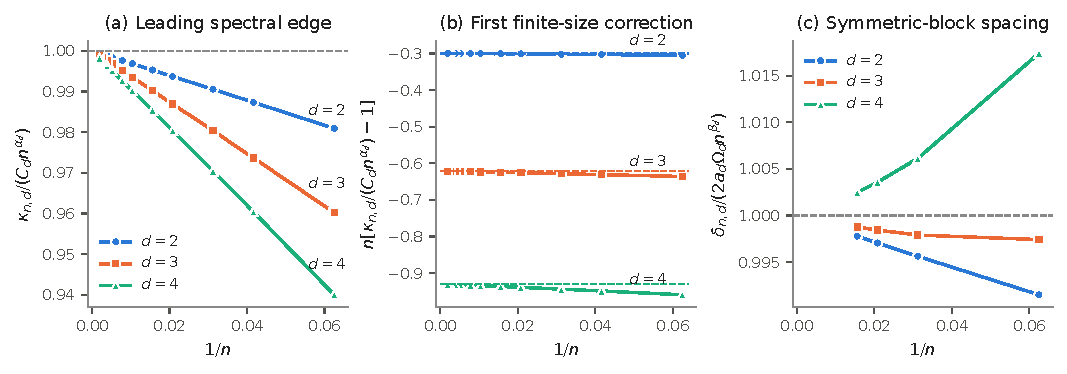
\includegraphics[width=\textwidth]{../figs/scaling.pdf}
\caption{Independent tests of the leading edge, first correction, and maximal-block spacing for $d=2,3,4$. (a) Perron root divided by $C_dn^{\alpha_d}$. (b) Scaled residual tending to $\alpha_d(1-\Omega_d)$. (c) Internal real-part gap divided by $2a_d\Omega_dn^{\beta_d}$. No coefficient is fitted. The $z=1$ values can be rescaled into the trace-nonincreasing domain. Positive iteration extends through $n=512$; dense arbitrary-precision spacings extend through $n=64$.}
\label{fig:scaling}
\end{figure*}

\section{Verification and numerical boundaries}
The reproducible bundle contains code, numerical tables, source records, and explicit checks. Exact symbolic characteristic polynomials were checked in six cases. The complete complex-fermion superoperator was compared with the frozen-set sign gauge for every $1\le d\le n\le4$, including random complex Hermitian $h$; maximum matrix residual was $1.96\times10^{-14}$. Additional checks include 4,134 integer CAR signs, spin intertwiners through seven modes, and 49 principal-submatrix identities.

The new observable calculation verifies the integer identities~\eqref{eq:identities} for all $2\le n\le7$, $1\le d\le n$ (27 cases). It propagates the full positive density matrix for $(n,d)=(4,2),(4,3),(5,2)$ and compares it with a population reduction retaining two marked modes. Maximum absolute propagation error is $1.34\times10^{-15}$; initial odd overlap and even--odd mixing matrix elements vanish. At $(4,3)$ a direct double-precision eigensolver splits a residual zero Jordan block, producing a $5.53\times10^{-6}$ error in the extracted even gap. That comparison is recorded as unsuitable, not as passed; the exact matrix identities and direct time propagation remain valid. The other two direct even-gap comparisons agree within $3.2\times10^{-14}$.

For the three larger dynamical examples, both exact two-channel formulas agree with marked-mode propagation. Fits on $5\le\gamma t\le8$ check the predicted tail rates to within $0.23\%$; fitted parameters do not enter the figures' theoretical curves. The spectral-amplitude approximations on $6\le\gamma t\le9$ differ from the propagated signals by at most $0.21\%$. At very long times, subtracting the stationary value limits double-precision signal accuracy, so no claim is based on indefinitely extending these tails.

Perron roots for $d=2,3,4$ at 11 sizes from $n=16$ to $512$, together with sizes $n-1,n-2$, use 99 converged logarithmic positive iterations. The maximum relative Collatz width is $2.00\times10^{-12}$. These are floating-point convergence diagnostics, not interval-arithmetic enclosures. Independent 50- and 70-digit spectra at $n=16,32,48,64$ give spacings agreeing within $10^{-10}$ after conversion to stored double precision. Agreement after rounding is not a certification of 50 accurate digits.

\bibliography{references}
\end{document}
